\documentclass[12pt,aspectratio=169]{beamer}

\usepackage{tikz}
\usetikzlibrary{arrows.meta}
\usepackage{bm}
\usefonttheme[onlymath]{serif}

\mode<presentation>{
  \usetheme{Boadilla}
}

\title{Delay Encryption}

\author[J. Burdges, L. De Feo]{Jeffrey Burdges\inst{1}, Luca De Feo\inst{2}}

\institute[W3F, IBM]{\inst{1}Web3 Foundation, Switzerland\\
  \inst{2}IBM Research Europe, Switzerland}

\date[Eurocrypt 2021]{Eurocrypt, October 19, 2021, Zagreb, Croatia}

\begin{document}

\setbeamertemplate{navigation symbols}{}
\frame[plain]{\titlepage}

\begin{frame}
  \Huge
  \centering
  
  How do you run a

  \bigskip

  sealed bid auction

  \bigskip

  \alert{without a trusted party?}
\end{frame}

{
  \setbeamercolor{background canvas}{bg=black}
  \begin{frame}[plain]
    \begin{tikzpicture}[remember picture,overlay]
      \node(pic)[at=(current page.center)] { 
        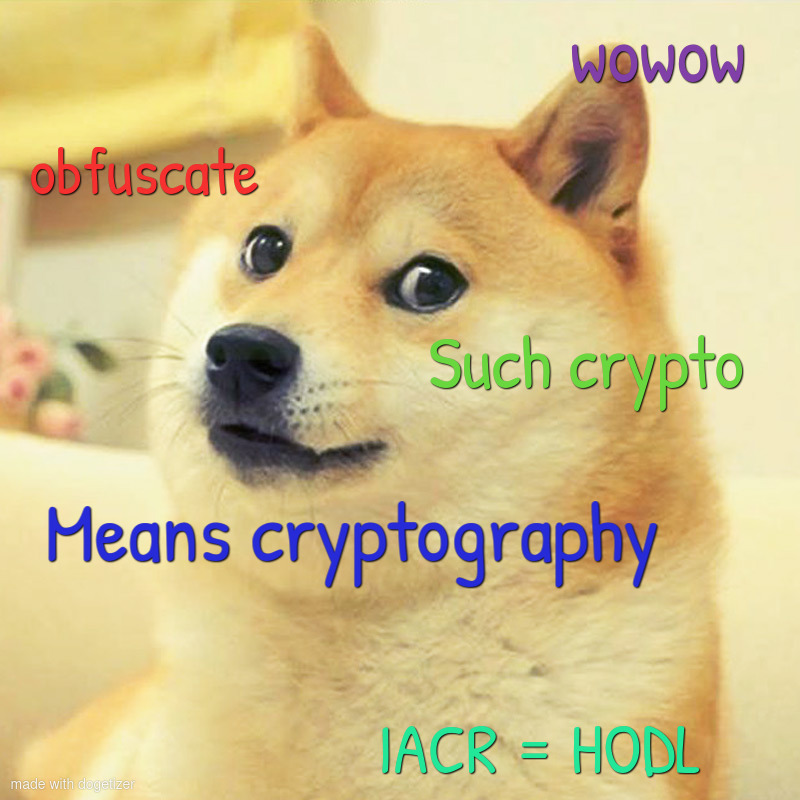
\includegraphics[height=\paperheight]{video/dogetizer-2021-10-12-2-38-14.jpg}
      };
    \end{tikzpicture}
  \end{frame}
  
  \begin{frame}[plain]
    \begin{tikzpicture}[remember picture,overlay]
      \node(pic)[at=(current page.center)] { 
        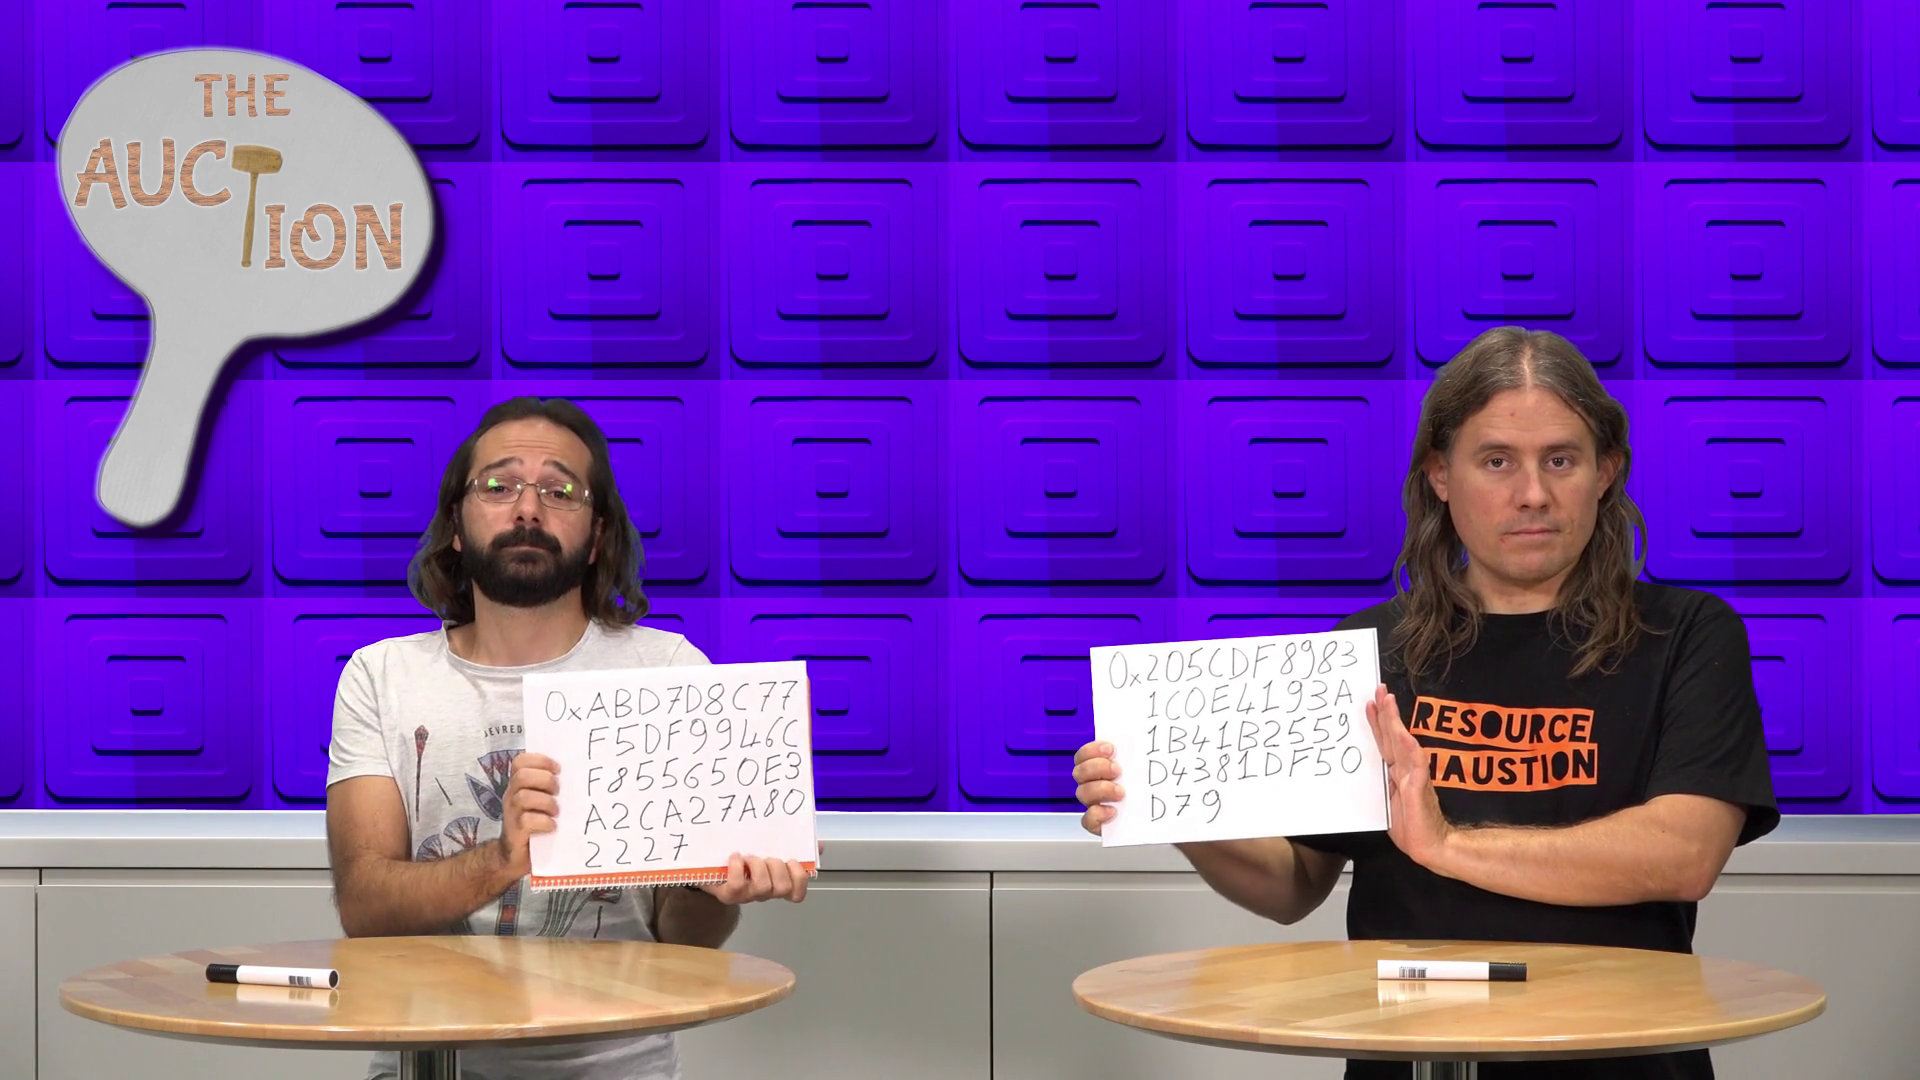
\includegraphics[width=\paperwidth]{commit.png}
      };
    \end{tikzpicture}
  \end{frame}
  
  \begin{frame}[plain]
    \begin{tikzpicture}[remember picture,overlay]
      \node(pic)[at=(current page.center)] { 
        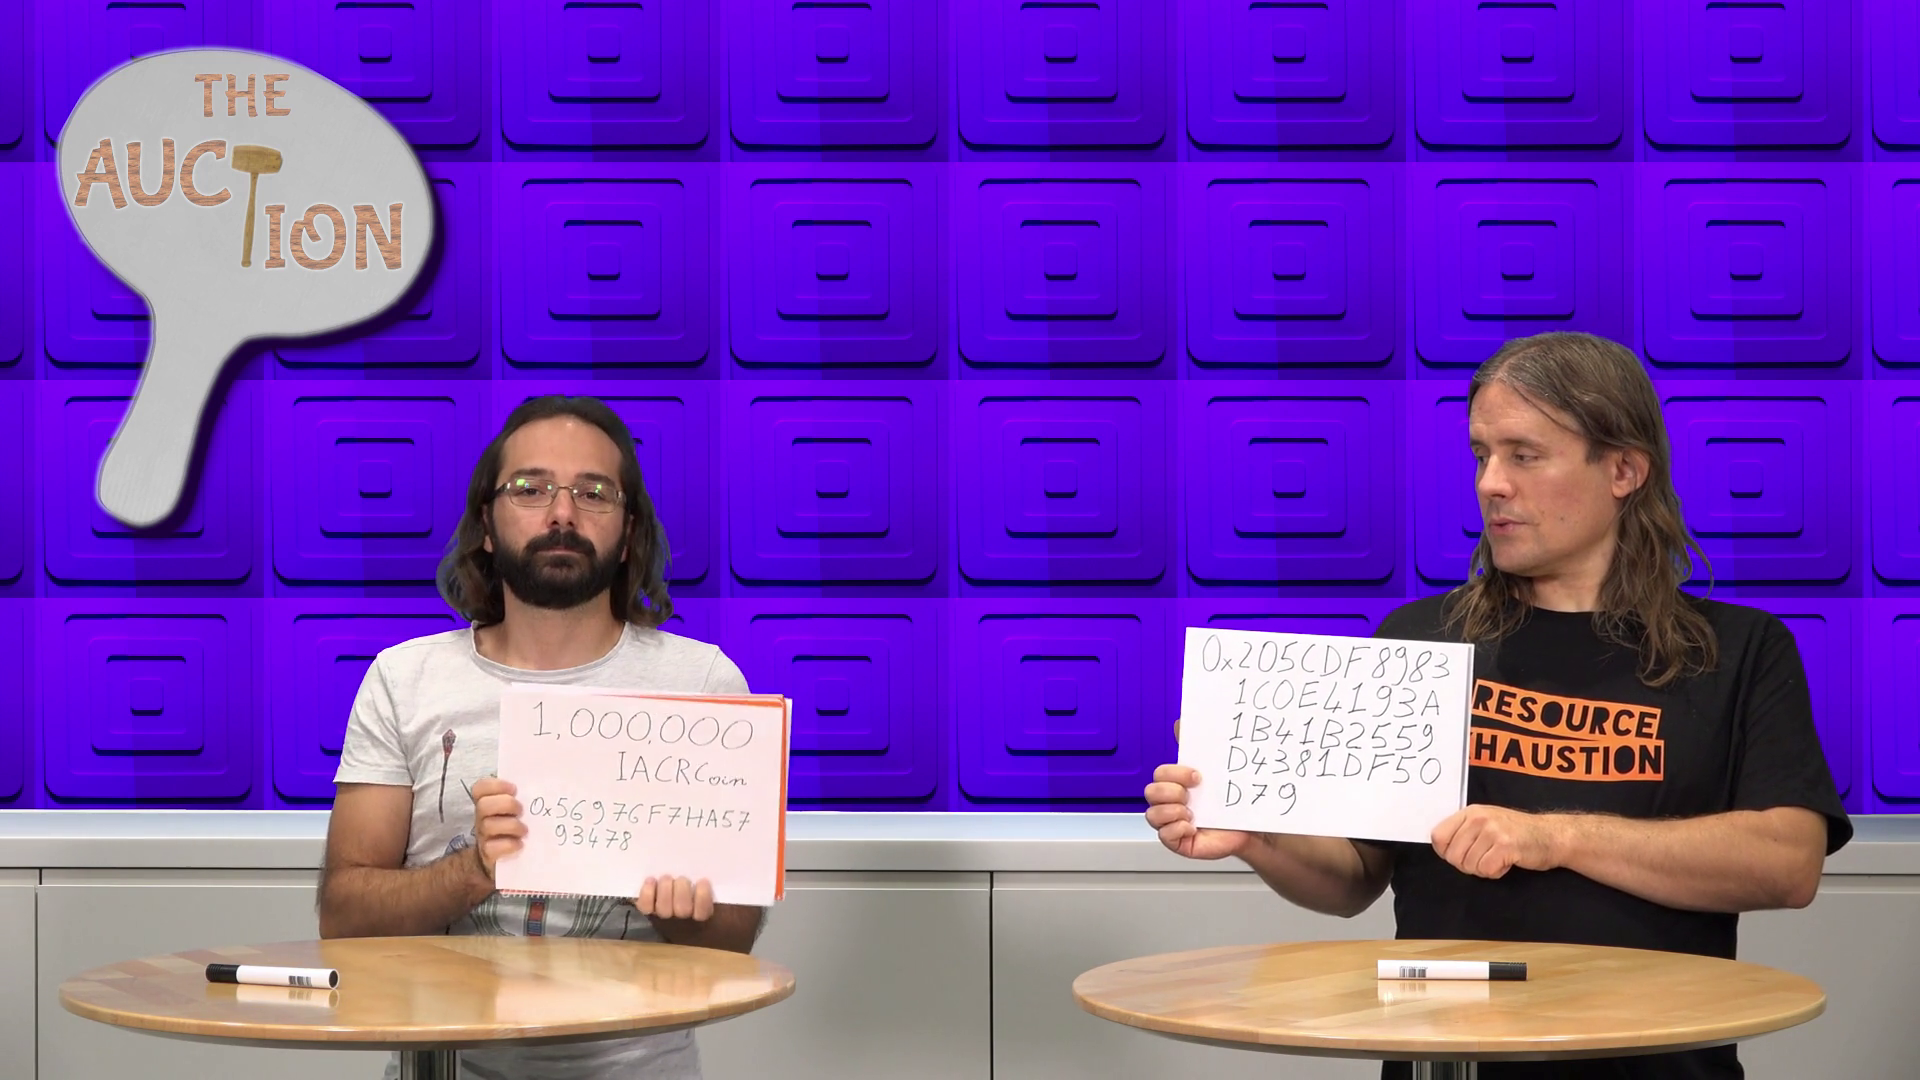
\includegraphics[width=\paperwidth]{reveal.png}
      };
    \end{tikzpicture}
  \end{frame}

  \begin{frame}[plain]
    \begin{tikzpicture}[remember picture,overlay]
      \node(pic)[at=(current page.center)] { 
        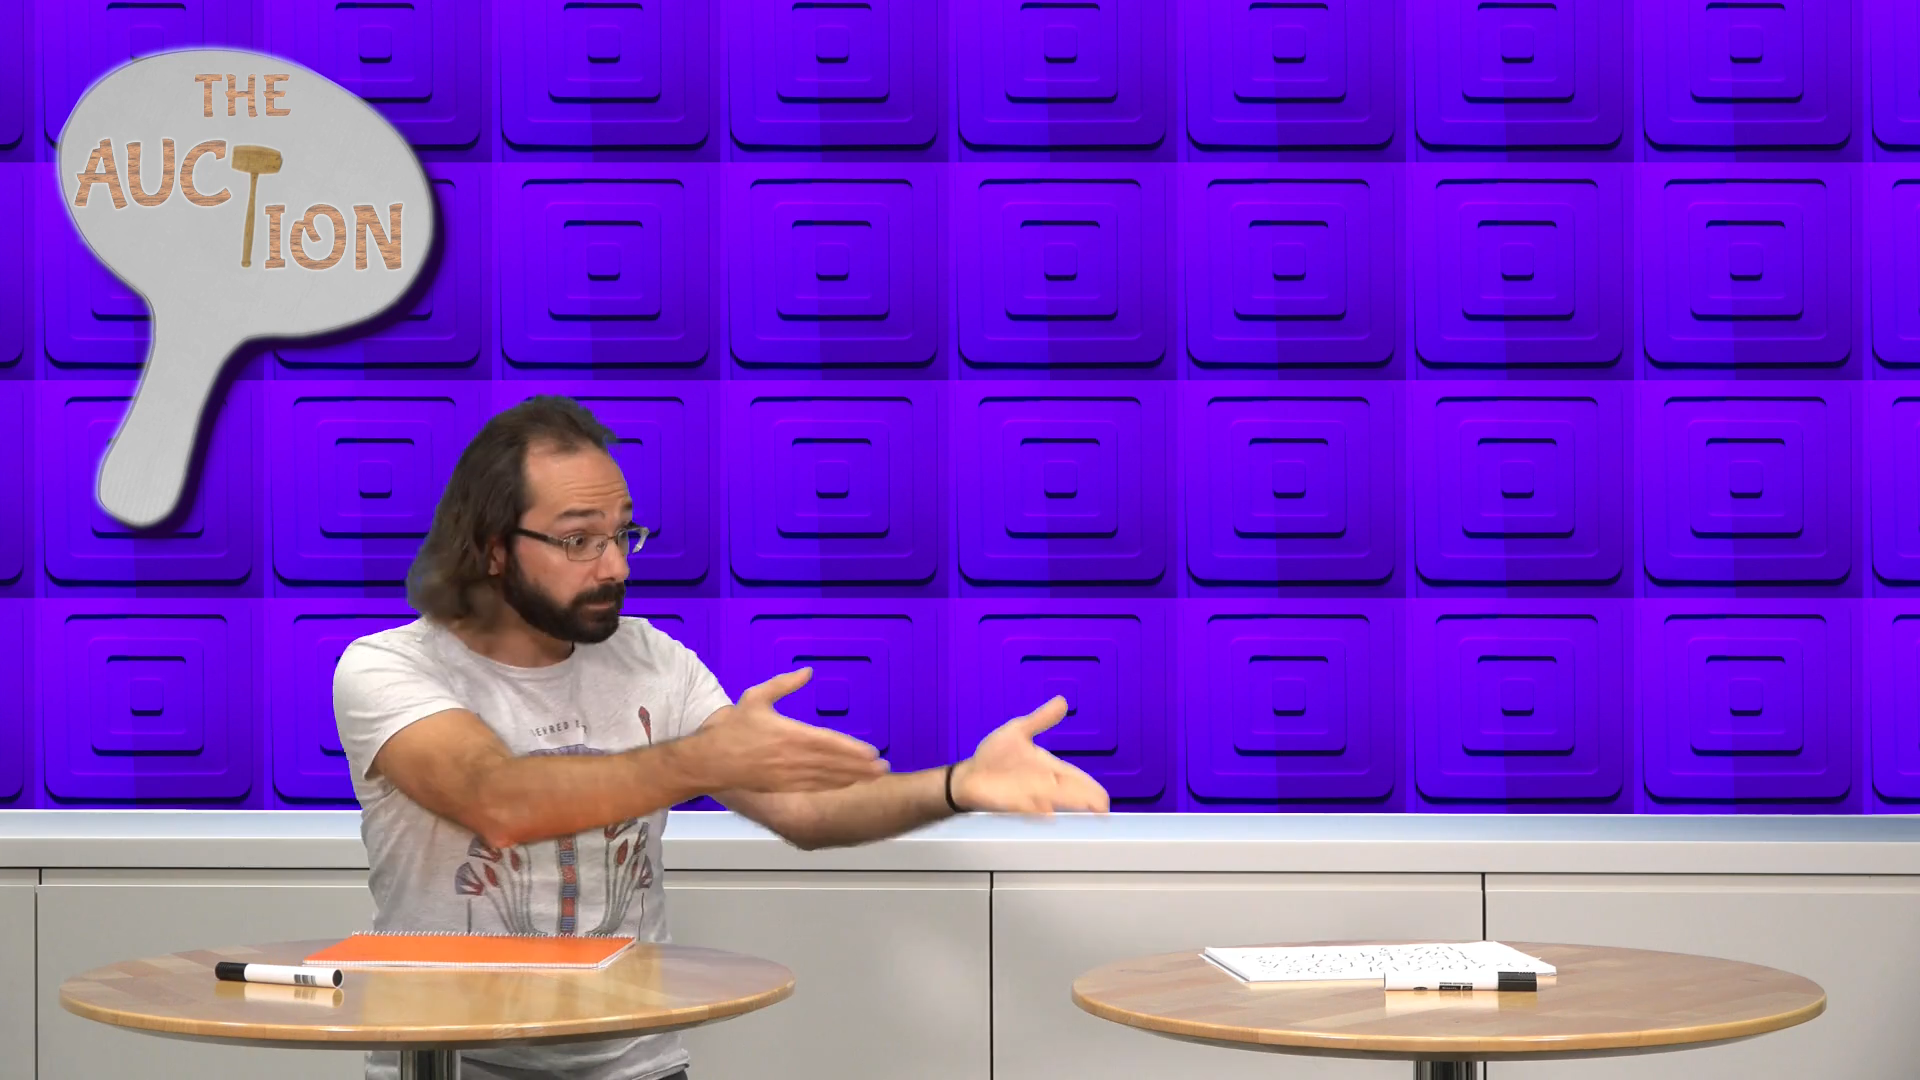
\includegraphics[width=\paperwidth]{complain2.png}
      };
    \end{tikzpicture}
  \end{frame}
}

\begin{frame}
  \Huge\centering
  Encrypt

  \bigskip
  \alert{to the Auction}
\end{frame}

\begin{frame}{Identity based encryption}
  \centering
  \begin{tikzpicture}
    \begin{scope}[color=white,every node/.style={fill=cyan,inner sep=3mm}]
      \node (keygen) at (0,0) {Keygen};
      \node (encrypt) at (-6,-3) {Encrypt};
      \node (extract) at (6,-3) {Extract};
      \node (decrypt) at (0,-6) {Decrypt};
    \end{scope}

    \begin{scope}
      \node (msk) at (4,-1) {msk};
      \node (pk) at (-4,-1) {pk};
      \node (msg) at (-6,-1) {msg};
      \node (ct) at (-4,-4.5) {ct};
      \node (sk) at (4,-4.5) {sk};
      \node (msg2) at (-6,-6) {msg};
      \node (id) at (0,-3) {
\includegraphics[height=3em]{video/doge.png}};
      \node[below of=id] {id};
    \end{scope}

    \draw[-latex] (keygen) edge (pk) edge (msk)
    (pk) edge (encrypt)
    (msg) edge (encrypt)
    (encrypt) edge (ct)
    (msk) edge (extract)
    (extract) edge (sk)
    (sk) edge (decrypt)
    (ct) edge (decrypt)
    (decrypt) edge (msg2)
    (id) edge (encrypt) edge (extract);
  \end{tikzpicture}
\end{frame}

\begin{frame}
  \Huge
  \begin{description}
    \setlength{\itemsep}{3em}
  \item[Solution 1:] Threshold Extraction
  \item[Solution 2:] \alert{Time Lock Extraction}
  \end{description}
\end{frame}

\begin{frame}{Boneh--Franklin IBE}
  \centering
  \def\doge{\raisebox{-.6em}{
\includegraphics[height=2em]{video/doge.png}}}
  \begin{tikzpicture}
    \begin{scope}[color=white,every node/.style={fill=cyan,inner sep=3mm}]
      \node (keygen) at (0,0) {Keygen};
      \node (encrypt) at (-6,-3) {$k = e(u\doge, mG_2)$};
      \node (extract) at (6,-3) {Extract};
      \node (decrypt) at (0,-6) {$k = e(m\doge, uG_2)$};
    \end{scope}

    \begin{scope}
      \node (msk) at (4,-1) {$m$};
      \node (pk) at (-4,-1) {$mG_2$};
      \node (msg) at (-6,-1) {$\mathrm{msg}$};
      \node (ct) at (-4,-5) {$\mathrm{Enc}_k(\mathrm{msg}), uG_2$};
      \node (sk) at (4,-5) {$m\doge$};
      \node (msg2) at (-6,-6) {$\mathrm{msg}$};
      \node (id) at (0,-3) {
\includegraphics[height=3em]{video/doge.png}};
    \end{scope}

    \draw[-latex] (keygen) edge (pk) edge (msk)
    (pk) edge (encrypt)
    (msg) edge (encrypt)
    (encrypt) edge (ct)
    (msk) edge (extract)
    (extract) edge (sk)
    (sk) edge (decrypt)
    (ct) edge (decrypt)
    (decrypt) edge (msg2)
    (id) edge (encrypt) edge (extract);
  \end{tikzpicture}
\end{frame}

\begin{frame}{Isogeny Based Delay Encryption}
  \centering
  \def\doge{\raisebox{-.6em}{
\includegraphics[height=2em]{video/doge.png}}}
  \def\iso{\textcolor{red!80!black}{\bm{\phi}}}
  \begin{tikzpicture}
    \begin{scope}[color=white,every node/.style={fill=cyan,inner sep=3mm}]
      \node (keygen) at (0,0) {Setup};
      \node (encrypt) at (-6,-3) {$k = e(u\doge, \iso G_2)$};
      \node (extract) at (6,-3) {Extract};
      \node (decrypt) at (0,-6) {$k = e(\iso\doge, uG_2)$};
    \end{scope}

    \begin{scope}
      \node (msk) at (4,-1) {$\iso$};
      \node (pk) at (-4,-1) {$\iso G_2$};
      \node (msg) at (-6,-1) {$\mathrm{msg}$};
      \node (ct) at (-4,-5) {$\mathrm{Enc}_k(\mathrm{msg}), uG_2$};
      \node (sk) at (4,-5) {$\iso\doge$};
      \node (msg2) at (-6,-6) {$\mathrm{msg}$};
      \node (id) at (0,-3) {
\includegraphics[height=3em]{video/doge.png}};
    \end{scope}

    \def\clock{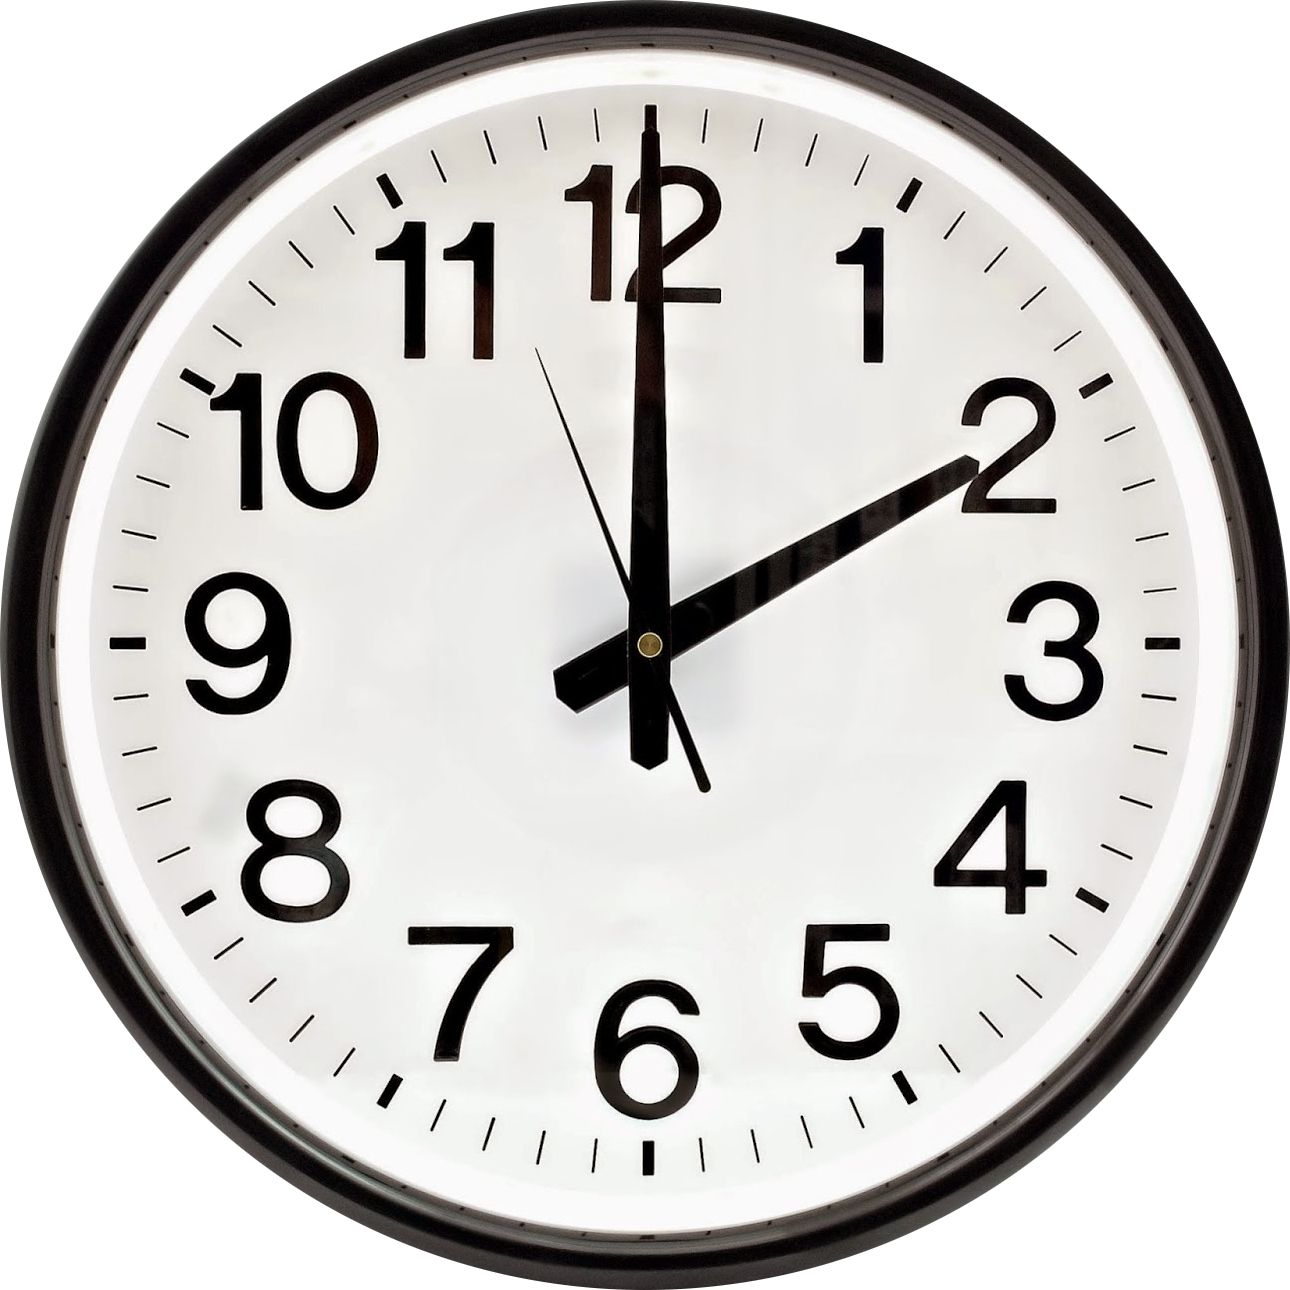
\includegraphics[height=2em]{video/clock.png}}
    \draw[-latex] (keygen) edge node {\clock} (pk) edge (msk)
    (pk) edge (encrypt)
    (msg) edge (encrypt)
    (encrypt) edge (ct)
    (msk) edge (extract)
    (extract) edge node {\clock} (sk)
    (sk) edge (decrypt)
    (ct) edge (decrypt)
    (decrypt) edge (msg2)
    (id) edge (encrypt) edge (extract);
  \end{tikzpicture}
\end{frame}

\begin{frame}
  \centering
  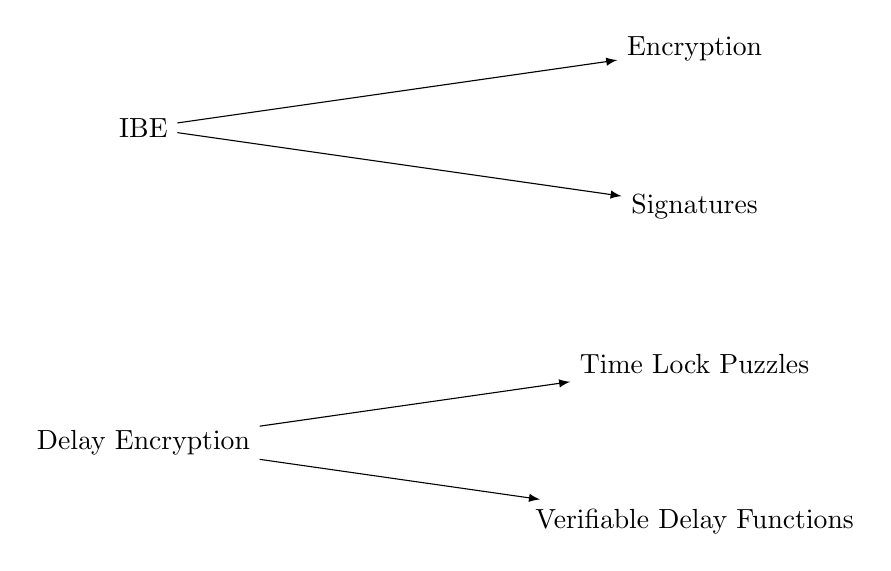
\begin{tikzpicture}
    \node (IBE) at (0,0) {IBE};
    \node (enc) at (7,1) {Encryption};
    \node (sig) at (7,-1) {Signatures};
    \node (DE) at (0,-4) {Delay Encryption};
    \node (TLP) at (7,-3) {Time Lock Puzzles};
    \node (VDF) at (7,-5) {Verifiable Delay Functions};

    \draw[-latex] (IBE) edge (enc) edge (sig)
    (DE) edge (TLP) edge (VDF);
  \end{tikzpicture}
\end{frame}

{
  \def\bl#1{\textcolor{blue}{#1}}
  \begin{frame}
    \centering
    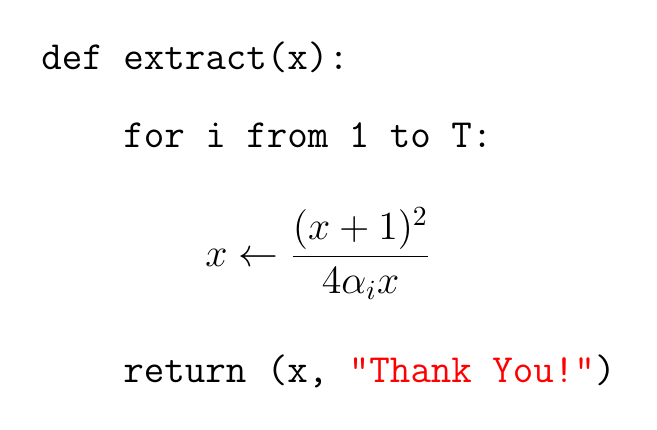
\begin{tikzpicture}
      \Large\tt
      \begin{scope}[anchor=west,x=2em]
        \node at (0,0) {\bl{def} extract(x):};
        \node at (1,-1) {\bl{for} i \bl{from} 1 \bl{to} T:};
        \node at (2,-2.5) {$\displaystyle x \leftarrow\frac{(x+1)^2}{4\alpha_i x}$};
        \node at (1,-4) {\bl{return} (x, \textcolor{red}{"Thank You!"})};
      \end{scope}
    \end{tikzpicture}
  \end{frame}
}

\end{document}
